% Select language used in document (ngerman or english). Automatically
% generated text is translated accordingly.
% use \selectthesislanguage in body.tex to switch to default language

%\documentclass[ngerman, paper]{mmt} % use for seminar paper
%\documentclass[ngerman, reviewversion]{mmt} % use for anonymized review version
%\documentclass[ngerman, bachelorthesis]{mmt} % use for Bachelor thesis
\documentclass[english, paper]{mmt} % use for Master thesis

\usepackage{mathptmx}
\usepackage{graphicx}
\usepackage{times}
\usepackage{subfig}
\usepackage{float}
\usepackage[utf8]{inputenc}
\usepackage[newfloat,langlinenos]{minted}
\usepackage{makecell}
\usepackage[toc,page]{appendix}
\usepackage{hyperref}
\hypersetup{
    colorlinks,
    citecolor=black,
    filecolor=black,
    linkcolor=black,
    urlcolor=black
}
\usepackage{breakurl}

\usepackage{amsmath}
\usepackage[autostyle,german=guillemets]{csquotes}

\usepackage{verbatim}

\newcommand{\detailtexcount}[1]{%
  \immediate\write18{texcount -merge -sum -q #1.tex > #1.wcdetail }%
  \verbatiminput{#1.wcdetail}%
}

% command for highlighting text that was generate with AI support
\newcommand{\aigen}[1]{\textcolor{blue}{#1}}

% moved to cls file. use \selectthesislanguage to switch to default language
%\usepackage[english,ngerman]{babel}

\usepackage{acronym}
\usepackage{abbrevs}
%% the following solves a bug in the abbrevs package, that adds an empty
%% space after the abbrev
\makeatletter
\renewcommand\maybe@space@{%
  % \@tempswatrue % <= this is in the original
  \maybe@ictrue % <= this is new
  \expandafter   \@tfor
    \expandafter \reserved@a
    \expandafter :%
    \expandafter =%
                 \nospacelist
                 \do \t@st@ic
  % \if@tempswa % <= this is in the original
  \ifmaybe@ic % <= this is new
    \space
  \fi
}
\makeatother
%%

%% ADD HERE YOUR CUSTOM CODE ENVIRONMENT AND SET DEFAULT VALUES %%
%% See https://mirror.kumi.systems/ctan/macros/latex/contrib/minted/minted.pdf
%% for
\newminted{csharp}{linenos,autogobble,fontsize=\footnotesize}
% \newminted{cpp}{linenos,autogobble,fontsize=\footnotesize}
%% Use it then with \begin{csharpcode} \end{csharpcode} or \begin{cppcode} \end{cppcode}

\usepackage{color}
\definecolor{lightgray}{rgb}{.9,.9,.9}
\definecolor{darkgray}{rgb}{.4,.4,.4}
\definecolor{purple}{rgb}{0.65, 0.12, 0.82}

\usepackage[url=false,authordate,bibencoding=auto,strict,noibid,backend=biber]{biblatex-chicago}
\bibliography{bibliography}
%% Add configuration options
\newabbrev{\authorname}{Felix Beer}
\newabbrev{\authormail}{fbeer.mmt-b2022@fh-salzburg.ac.at}
\newabbrev{\titlename}{An Overview of 3D Object Reconstruction Diffusion Models}
\newabbrev{\advisor}{DI Gerlinde Emsenhuber}
%\newabbrev{\secondadvisor}{Titel Vorname Nachname}
\newabbrev{\thesisdate}{dd.mm.yyyy}
\newabbrev{\thesisrepo}{https://github.com/felixbeer/3d-diffusion-models-paper}
\newabbrev{\keywordsenglish}{word1, word2, word3}
\newabbrev{\keywordsgerman}{wort1, wort2, wort3}


%% Paper title.

\title{\titlename}

%% This is how authors are specified in the conference style

%% Author
\author{ \authorname\\ \scriptsize \authormail \\ \scriptsize
\ifmmtlanguagegerman FH Salzburg \else Salzburg University of Applied Sciences \fi
}

%% A teaser figure can be included as follows, but is not recommended since
%% the space is now taken up by a full width abstract.
%\teaser{
%  \includegraphics[width=1.5in]{sample.eps}
%  \caption{This can be a teaser image of the thesis.}
%}

%% Abstract section for paper format.
\abstract{
    \ifmmtlanguagegerman
        \selectlanguage{ngerman}
        \input{kurzfassung}
    \else
        \selectlanguage{english}
        %%%%% IMPORTANT: do not use the acronym package here, but only in the main text. I.e., define acronyms manually here for now. %%%%%

% Lorem ipsum dolor sit amet, consectetur adipiscing elit. Aenean venenatis nulla vestibulum dignissim molestie. Quisque tristique tortor vitae condimentum egestas. Donec vitae odio et quam porta iaculis ut non metus. Sed fermentum mauris non viverra pretium. Nullam id facilisis purus, et aliquet sapien. Pellentesque eros ex, faucibus non finibus a, pellentesque eu nibh. Aenean odio lacus, fermentum eu leo in, dapibus varius dolor. Lorem ipsum dolor sit amet, consectetur adipiscing elit. Proin sit amet ornare velit. Donec sit amet odio eu leo viverra blandit. Ut feugiat justo eget sapien porttitor, sit amet venenatis lacus auctor. Curabitur interdum ligula nec metus sollicitudin vestibulum. Fusce placerat augue eu orci maximus, id interdum tortor efficitur.

    \fi
}

%%%%%%%%%%%%%%%%%%%%%%%%%%%%%%%%%%%%%%%%%%%%%%%%%%%%%%%%%%%%%%%%
%%%%%%%%%%%%%%%%%%%%%% START OF THE PAPER %%%%%%%%%%%%%%%%%%%%%%
%%%%%%%%%%%%%%%%%%%%%%%%%%%%%%%%%%%%%%%%%%%%%%%%%%%%%%%%%%%%%%%%%

\begin{document}
% TODO switch for english, german
\selectthesislanguage

\pagenumbering{gobble}

 % group open
\ifmmtpaper
    \begingroup
    % is required because paper template messes with sizes
    \fontsize{12}{18}\selectfont
    \setlength{\parindent}{0pt}
    \setlength{\parskip}{5pt plus 2pt minus 1pt}
    \sectionfont{\fontsize{14}{15}\selectfont}
\fi

\ifmmtreviewversion
    \titlename
\else
    \input{title}
\fi

    \onecolumn

    \pagenumbering{roman}

\ifmmtpaper % does not need affidavit
\else \ifmmtreviewversion
      \else
        \newpage
        \input{affidavit}  % comment out for expose
      \fi
\fi
% group closing
\ifmmtpaper
\endgroup
\fi


\ifmmtpaper \else  % paper does not need this stuff

    \newpage
    \selectlanguage{ngerman}
    \section*{Kurzfassung}
    \input{kurzfassung}
    \ifmmtmasterthesis

    \vspace*{0.5cm}
    \textbf{Schlüsselwörter:~} \keywordsgerman
    \fi
    \newpage
    \selectlanguage{english}
    \section*{Abstract}
    %%%%% IMPORTANT: do not use the acronym package here, but only in the main text. I.e., define acronyms manually here for now. %%%%%

% Lorem ipsum dolor sit amet, consectetur adipiscing elit. Aenean venenatis nulla vestibulum dignissim molestie. Quisque tristique tortor vitae condimentum egestas. Donec vitae odio et quam porta iaculis ut non metus. Sed fermentum mauris non viverra pretium. Nullam id facilisis purus, et aliquet sapien. Pellentesque eros ex, faucibus non finibus a, pellentesque eu nibh. Aenean odio lacus, fermentum eu leo in, dapibus varius dolor. Lorem ipsum dolor sit amet, consectetur adipiscing elit. Proin sit amet ornare velit. Donec sit amet odio eu leo viverra blandit. Ut feugiat justo eget sapien porttitor, sit amet venenatis lacus auctor. Curabitur interdum ligula nec metus sollicitudin vestibulum. Fusce placerat augue eu orci maximus, id interdum tortor efficitur.

    \ifmmtmasterthesis

    \vspace*{0.5cm}
    \textbf{Keywords:~} \keywordsenglish
    \fi
    \selectthesislanguage

    \newpage
    \tableofcontents

    \newpage
    \listoffigures
    \listoflistings
    \listoftables
    \input{abbreviations}

\fi


\mmtcolumnmode % switch back to column formatting of stylesheet

\maketitle % used for paper formatting

\ifmmtpaper\else
\pagestyle{headings}
\fi
\pagenumbering{arabic}


% put environments that should be ignored by texcount here, e.g., here listing for code

%TC:envir listing [] ignore

%for reference to this section
\section{Introduction}
\label{section:Introduction}
In today's world, nearly every industry uses 3D models to visually represent objects or environments. Whether for entertainment, development, or research, 3D models are essential tools for understanding complex concepts and ideas.

Creating these models is a time-consuming and costly process that requires skilled artists and designers, especially when compared to taking pictures or recording videos with cameras or smartphones. However, recent advancements in Generative 3D AI have made it possible to generate 3D models from a single image. This process, known as 3D object- or mesh-reconstruction, has the potential to transform and partially automate the creation and use of 3D models.

Some examples include the newly released TripoSR (\textcite{tochilkin_triposr_2024}) as well as established models like Zero-1-to-3 (\textcite{liu_zero-1--3_2023}), One-2-3-45 (\textcite{liu_one-2-3-45_2023}), and One-2-3-45++ (\textcite{liu_one-2-3-45_2023-1}).

This paper provides an overview of the various approaches and models used for 3D mesh reconstruction, including a comparison of their performance and visual results.
Furthermore, it discusses the different strategies like voxel-based \autocite{zhirong_wu_3d_2015}, point cloud-based \autocite{charles_pointnet_2017}, and mesh-based \autocite{wang_pixel2mesh_2018} methods.
It also explores the underlying methods and concepts like convolutional neural networks and neural radiance fields \autocite{mildenhall_nerf_2021} used in modern neural network-based models.
Finally, it offers a brief look at use cases and applications that benefit the most as well as 3D-model datasets such as Objaverse-XL \autocite{deitke_objaverse-xl_2023} and their impact on model training.
% \section{System Overview}
% Provide a high level overview of your system, approach, etc.
% Describe features, user interfaces, provide screenshots.
% What does a user do with your application/system/interaction method?

% \begin{listing}[H]
%     \begin{csharpcode}
%     for (var item in myList)
%     {
%         Console.WriteLine($"Fancy syntax highlighting for {item}");
%     }
%     \end{csharpcode}
%     \caption{Example of a listing.}
%     \label{lst:example}
% \end{listing}

% See code \ref{lst:example} for high efficiency code.

\section{Concepts and Functionality}
To understand the process of 3D mesh reconstruction, it is essential to understand the underlying concepts and techniques used in the field. This section provides a quick overview of the different methods and approaches used to generate 3D models from 2D images.

\subsection{Shape from Shading}
Starting with shape from shading, this is the most basic technique used to estimate the shape of an object from a single image, which dates back to the late 80s (\textcite{horn_shape_1989}).
The basic idea is to use the shading information in the image to infer the 3D structure of the object. This is done by assuming that the object gets illuminated by a single light source and that the surface of the object is Lambertian, meaning that the surface reflects light uniformly in all directions. This by itself is a strong assumption, as most real-world objects are not perfectly Lambertian.
Estimating surface normals at each point on the object involves using the intensity of the reflected light and then integrating the normals to estimate the object's depth. This technique was one of the first to show that basic 3D shape information could be recovered from a single image and has since inspired many other techniques for 3D reconstruction.
\begin{figure}
    \centering
    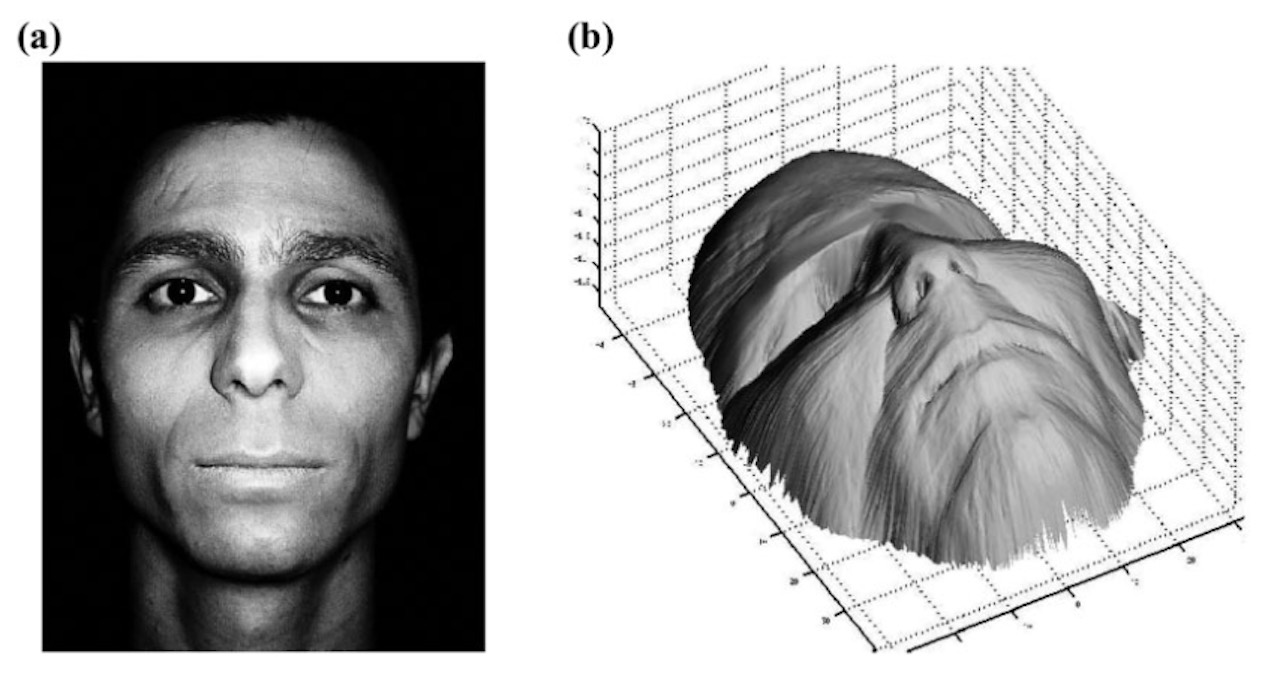
\includegraphics[width=0.5\linewidth]{images/shape_from_shading.jpg}
    \caption{Shape from shading \autocite{horn_shape_1989}}
    \label{fig:shape_from_shading}
\end{figure}

\subsection{Multi-view Stereo}
Before the appearance of deep learning, multi-view stereo was the most common technique used for 3D reconstruction.
The basic idea is the concept of Structure from motion (SfM) and can not be sourced to a single publication but rather a collection of works.
\textcite{ullman_interpretation_1997} were among the first ones to describe the process in a computational context.

\paragraph
"[…] the structure from motion theorem which states that the structure of 4 non-coplanar points is recoverable from 3 orthographic projections." \autocite{ullman_interpretation_1997}

\paragraph
In other words, SfM describes the use of multiple images of an object taken from different angles to estimate the 3D structure of the object.
This is done by first estimating the camera parameters for each image and then using these parameters to triangulate the 3D points in the scene.

\textcite{furukawa_accurate_2010} proposed a robust and efficient algorithm based on many well established techniques like Difference of Gaussians (DoG) and Harris corner detection for feature detection and matching.

The whole process of multi-view stereo has also gained great relevance in augmented and virtual reality to reconstruct and map the environment in real-time.

\subsection{Convolutional Neural Networks}
Convolutional Neural Networks (CNNs) have empowered the field of computer vision and have found applications in many areas, including 3D mesh reconstruction.
CNNs are a type of deep learning models that are especially good at working with image data. They are designed to automatically and adaptively learn spatial hierarchies of features from the data.
\paragraph{}
AlexNet by \textcite{krizhevsky_imagenet_2012} was one of the first applications of CNNs to image classification and delivered a significant performance improvement: “On the test data, we achieved top-1 and top-5 error rates of 37.5\% and 17.0\% which is considerably better than the previous state-of-the-art.” \autocite{krizhevsky_imagenet_2012}
Top-1 and top-5 error rates are common metrics used to evaluate the performance of image classification models. The top-1 error rate is the percentage of images for which the correct label is not in the top-1 predicted labels, while the top-5 error rate is the percentage of images for which the correct label is not in the top-5 predicted labels.

\subsection{Generative Adversarial Networks}
Generative Adversarial Networks (GAN) \autocite{goodfellow_generative_2014} are a type of deep learning model that consists of two neural networks: a generator and a discriminator. The generator is responsible for generating new data samples, while the discriminator is responsible for distinguishing between real and generated data samples. The two networks are trained together in competition, where the generator tries to generate realistic data samples to fool the discriminator, and the discriminator tries to distinguish between real and generated data samples.
\paragraph{}
In the context of 3D mesh reconstruction, CNNs and GANs are often used together to generate 3D models from 2D images. The CNN is used to extract features from the input image, and the GAN is used to generate the 3D model from these features. One example of this is the Pixel2Mesh++ model by \textcite{wen_pixel2mesh_2019}.

\subsection{Neural Implicit Functions}
...
\textcite{park_deepsdf_2019}
\textcite{mildenhall_nerf_2021}

\section{Models}

In the recent years several models have been developed to generate 3D models from 2D images. Some of the most prominent models include:

\subsection{Pixel2Mesh}
Pixel2Mesh is a model developed by \textcite{wang_pixel2mesh_2018}.
It is built with two main components. The image feature network which is a convolutional neural network (CNN) that extracts perceptual features from the input image. The second component is a cascaded mesh deformation network which is a graph-based convolution network.

A graph-based convolution network differs from traditional CNNs in that it operates on a graph rather than a grid. In the context of Pixel2Mesh, the graph represents the 3D mesh model with vertices and edges.

\paragraph{}
The Pixel2Mesh model works in the following steps:
\begin{enumerate}
    \item The input image is passed through the image feature network to extract features.
    \item The cascaded mesh deformation network initializes with an ellipsoid mesh model.
    \item The features extracted from the image are then taken to refine the shape of the mesh model.
    \item The mesh model gets refined iteratively in 3 blocks, with each iteration refining the shape and increasing the mesh resolution. (see Figure \ref{fig:pixel2mesh})
    \item The vertex positions get estimated each step, which are then used to look up the features from the image feature network for the next iteration.
\end{enumerate}
\begin{figure}
    \centering
    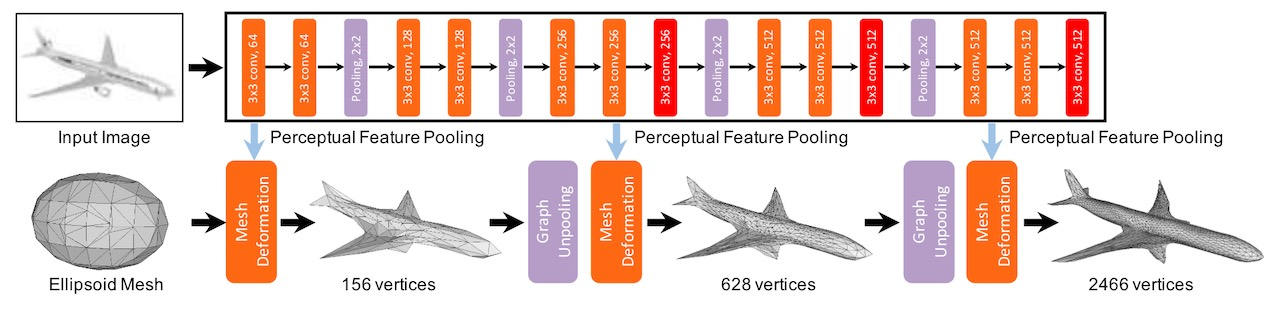
\includegraphics[width=1\linewidth]{images/pixel2mesh.jpg}
    \caption{Pixel2Mesh Pipeline \autocite{horn_shape_1989}}
    \label{fig:pixel2mesh}
\end{figure}

\subsection{Pixel2Mesh++}
Pixel2Mesh++ \autocite{wen_pixel2mesh_2019} is an extension of the original Pixel2Mesh model. It improves the performance by incorporating a Generative Adversarial Network (GAN) like approach.

\subsubsection{One-2-3-45}
This model was developed by \textcite{liu_one-2-3-45_2023-1}...

\subsubsection{Zero-1-to-3}
Zero-1-to-3 is a model developed by \textcite{liu_zero-1--3_2023}...
\subsubsection{TripoSR}
TripoSR is a model developed by \textcite{tochilkin_triposr_2024}...

\subsection{Comparison}
Result comparison between models both visually and in terms of performance.

\section{Applications of 3D Mesh Reconstruction}
As the field is still relatively new, no mainstream applications have been established yet. However, the potential is great and some possible applications have already been identified.

\subsection{Development and Entertainment}
The most prominent application of 3D mesh reconstruction could be in the development and entertainment industry. The ability to generate 3D models from 2D images could revolutionize the asset creation process.
This could be especially beneficial for indie developers or small studios that do not have the resources to create high-quality 3D models from scratch. The generated models could be used in video games, movies, animations, and other forms of media. This could significantly reduce the time and cost associated with creating 3D assets, allowing developers and animators to focus on other aspects of their projects. (see Figure \ref{fig:one-2-3-4-5-plus-plus-demo})
\begin{figure}
    \centering
    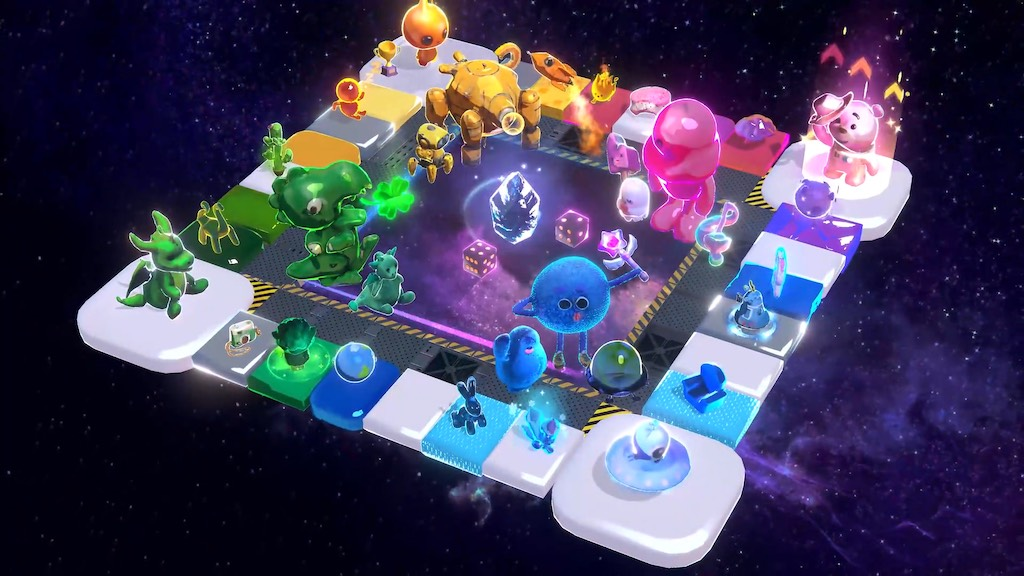
\includegraphics[width=1\linewidth]{images/one-2-3-45++_demo.jpg}
    \caption{Models generated by One-2-3-45++ \autocite{liu_one-2-3-45_2023-1}}
    \label{fig:one-2-3-4-5-plus-plus-demo}
\end{figure}

\subsection{Medical}

\subsection{Other Applications}

\subsubsection{Cultural Heritage}

% \section{Ethical Implications}
% Even though all the advancements in the field of 3D mesh reconstruction are promising, they also raise quite a few concerns.

% \subsection{Environmental Impact}
% Estimations of energy consumption for training as well as execution of models.

% \subsection{Training Data}
% The sources of training data. Looking at datasets like Objaverse-XL \autocite{deitke_objaverse-xl_2023} and their sources.

% \subsection{Privacy Concerns}

% \subsection{Cultural Sensitivity}
% It is important that the models are actually representative of the cultures, especially when generating models of people or culturally significant objects.

% \subsection{Implications of Estimations and Hallucinations}
% It is usually necessary for these models to estimate not seeable parts of the object. This can lead to hallucinations and other artifacts in the generated models.

% \section{Implementation}
% Provide implementation details such as the used software and our software architecture, highlight your own solutions to encountered difficulties. Describe relevant iterations of your implementation.

% Describe your methodology. How did you evaluate your work? Why did you choose this methodology? Present results of your evaluation here.

\section{Discussion and Future Direction}
Discussion of results and their implications. What are the limitations current works? What are the next steps in this research area?
% Discuss your results to answer your research question. Does your data support you hypotheses? Put your results into perspective by situating it in the research field/related work.

\section{Conclusion}
% Summarize your work, outline limitations and future work.

% \section{Formatierung}
% \label{section:Formatting}

% Text mit beliebigen Sonderzeichen in UTF-8 ohne BOM \ldots
% ,
% \textbf{hervorgehobener Text},
% \texttt{void}\footnote{Fußnote 1},
% mathematische Formel im Text $\sum_{i=0}^n i^2$
% \ldots

% Referenz auf Unterabschnitt \ref{subsection:Coding} der Arbeit, automatisch richtig nummeriert.

% \textcite[]{Mulloni:2010} für einen einen Literaturverweis im laufenden Text.

% Literaturverweise sind essentiell für eine wissenschafliche Arbeit. \autocite[]{McConnell:2004:CCS:1096143}.

% Achtung: nur zitierte Literatur wird im Literaturverzeichnis
% angeführt.\footnote{Fußnote 2}


% Wir verwenden \LaTeX\footnote{ \url{http://en.wikibooks.org/wiki/LaTeX}} -- und das
% ist keine Quelle, sondern blos eine URL.

% \subsection{Figures machen was sie wollen}

% % h = try to place the figure Here
% % t = try to place the figure at the Top of a page
% % p = try to place this figure along with others on a separate Page
% % Note that LaTeX has a sophisticated ranking algorithm to place figures.
% % It is not always easy to accept LaTeX's placing but it is harder doing it
% % manually. Just let it go ;-)
% \begin{figure}[!ht]
% 	\centering
% 	\subfloat[Das Julia Fraktal]{
% 		\includegraphics[width=0.75\linewidth]{images/Julia-Fractal.png}
% 		%for reference of this subfigure only
% 		\label{subfigure:Julia-Fractal}
% 	}
% 	\qquad
% 	\subfloat[Noise für Tinteneffekte]{
% 		\includegraphics[width=0.75\linewidth]{images/Perlin-Coherent.png}
% 		%for reference of this subfigure only
% 		\label{subfigure:Perlin-Coherent}
% 	}
% 	\caption[
% 		Verschiedene Pixelgraphiken\newline
% 		% source url given in the table of figures
% 		\small\texttt{https://mediacube.at/wiki/}
% 	]{
% 		Verschiedene Pixelgraphiken
% 	}
% 	%for reference to all subfigures
% 	\label{figure:PixelImages}
% \end{figure}

% Unterstützte Pixelgraphikformate: PNG, JPEG, PDF.
% Angabe von height oder width meist wichtig.

% Referenz auf Abbildung \ref{figure:PixelImages} mit allen Teilbildern.
% Referenz auf Unterabbildung \ref{subfigure:Julia-Fractal}.

% %figure* stretches figure over both columns
% \begin{figure*}[t]
% 	\centering
% 	\includegraphics[width=0.9\textwidth]{images/KappaGamma.pdf}
% 	\caption{
% 		Vektorgraphik mit \LaTeX\ Beschriftung ($\kappa$, $\gamma$)
% 	}
% 	%for reference to this figure
% 	\label{figure:KappaGammaTau}
% \end{figure*}

% Referenz auf Abbildung \ref{figure:KappaGammaTau}.

% Bei Vektorgraphik mit \LaTeX\ Beschriftung keine Skalierung mit width oder height verwenden.

% Vektorgraphik mit \LaTeX\ Beschriftung kann etwa mit \texttt{ipe} erstellt werden.

% Unterstütztes Vektorgraphikformat: PDF. EPS muss konvertiert werden.


% \subsection{Unterabschnitt 2}
% %for references to this subsection
% \label{subsection:Coding}

% \begin{listing}[H]
%     \begin{csharpcode*}{firstnumber=10}
%         while (true)
%         {
%             // Ignition
%         }
%     \end{csharpcode*}

%     \caption{Example of another listing.}
%     \label{lst:Main}
% \end{listing}

% Wie man in Listing \ref{lst:Main}, kann man die erste Zeilennummern im Listing absichtlich ändern, hier z.B. auf 10. Beachte, dass man hier chsarpcode* als Umgebung nutzt, um neben
% den Default-Settings zusätzliche Einstellungen zu tätigen.

% \subsubsection{Unterunterabschnitt i}

% Wörtliches Zitat:
% %select proper language if not in German
% \selectlanguage{english}
% \begin{quote}
% ``Erwin Unruh discovered that templates can be used to compute
% something at compile time. [...] The intriguing part of this exercise, however, was that the production of the prime numbers was performed by the compiler during the compilation process and not at run time.''

% \autocite[305]{Bosch2014}
% \end{quote}
% %select German again or the language that you were using before (note ngerman stands for New German)
% %\selectlanguage{ngerman}
% \selectthesislanguage


% \subsection{Unterabschnitt b}

% \begin{enumerate}
% 	\item Punkt 1
% 	\begin{enumerate}
% 		\item Unterpunkt 1
% 		\item Unterpunkt 2
% 	\end{enumerate}
% 	\item Punkt 2
% \end{enumerate}

% \begin{itemize}
% 	\item Punkt 1
% 	\begin{itemize}
% 		\item Unterpunkt 1
% 		\item Unterpunkt 2
% 	\end{itemize}
% 	\item Punkt 2
% \end{itemize}


% \subsection{Unterabschnitt c}

% \begin{table}[ht]
% 	\centering
% 	\begin{tabular}{r|rrr}
% 		    & $i$ & $j$ & $k$ \\ \hline
% 		$i$ &$-1$ & $k$ &$-j$ \\
% 		$j$ &$-k$ &$-1$ & $i$ \\
% 		$k$ & $j$ &$-i$ &$-1$
% 	\end{tabular}
% 	\caption{
% 		Multiplikationstabelle für Quaternionen
% 	}
% 	\label{table:Quaternions}
% \end{table}

% Referenz auf Tabelle \ref{table:Quaternions}.

% \section{Abschnitt 2}
% \label{section:MathematicalStuff}

% Sei $f(x)$ eine stetige Funktion, so ist die \textbf{Fourier Transformierte}
% $F(\omega)$ wie folgt definiert:
% \begin{equation}
% \label{equation:FourierDefinition}
% 	F(\omega) = \int_{-\infty}^{\infty} f(x) e^{-i\omega t} dt
% \end{equation}

% Referenz auf mathematische Gleichung (\ref{equation:FourierDefinition}).

% Unnummerierte Gleichung:
% \begin{equation*}
% 	e^{i\varphi} = \cos\varphi + i \sin\varphi
% \end{equation*}
% %you may also use \[ \] instead of \begin{equation*} and \end{equation*}

% Gleichungssystem:
% \begin{eqnarray}
% 	g(x) = f(x - x_0) & \Leftrightarrow &
% 		G(\omega) = F(\omega) e^{-i\omega x_0} \\
% 	g(x) = f(x) e^{i\omega_0 x} & \Leftrightarrow &
% 		G(\omega) = F(\omega - \omega_0)
% \end{eqnarray}
 % the main text

%\input{acknowledgements}

\ifmmtpaper

\printbibliography

\else % only use the following for thesis format

\newpage
\printbibliography

\fi


 % group open
\ifmmtpaper
\begingroup
    % is required because paper template messes with sizes
    \fontsize{12}{18}\selectfont
    \setlength{\parindent}{0pt}
    \setlength{\parskip}{5pt plus 2pt minus 1pt}
    \sectionfont{\fontsize{14}{15}\selectfont}
\fi

\ifmmtpaper\else % nicht im paper

\newpage
\onecolumn
\begin{appendices}


\section{AI Methodology}

\textbf{You can delete the explanatory text in this section and add your AI documentation.}

Document in this section, how AI was utilized to support the creation of this seminar paper or thesis. Which tools were used? Which steps of the thesis creation were supported (e.g., brain storming, literature search, quality analysis of papers, text generation, text summaries, paraphrasing, spellchecking, ...). If generative AI was utilized (e.g., ChatGPT, CoPilot), also provide key text prompts that influenced the thesis.

In the following, list each tool and provide a brief description how the tool as utilized. For each tool, estimate in \% of the word count of the thesis, how much text was generated/modified/etc. by the AI tool. For the practical part of the thesis, estimate the \% of the results (e.g., code) was generated/mofidied/etc. by the AI tool. If a generative AI was used, provide exemplary prompts.

There is no requirement to highlight text in the thesis.

This section should have a maximum length of 2 pages.

\subsection{DeepL} % example tool
I used the tool (\url{https://addressoftool.com}) to [paraphrase|translate|...] text for this work.  I estimate that XX \% of the text was paraphrased with this tool.

\subsection{Copilot}
I used Copilot (\url{https://addressoftool.com}) to learn how to utilize RUST as a new programming language. ....
I estimate taht XXX \% of the source code was created with this tool.

\subsection{AI Tool 2}
... document tool usage ...

\subsection{Prompts}
I utilized the generative AI \url{https://bot.com} to create drafts for texts, support brainstorming, ...

... list exemplary prompts here ...

%\renewcommand{\thesubsection}{\Alph{subsection}}

% DIESEN TEIL NICHT LÖSCHEN ODER ÄNDERN == BEGINN
%\fi % end if for the if \ifmmtreviewversion
\end{appendices}
% DIESEN TEIL NICHT LÖSCHEN ODER ÄNDERN == ENDE


\fi

% group closing
\newpage

This work has the following word count (counted by texcount):
%TC:ignore
\detailtexcount{body}
%TC:endignore

\end{document}
